\section{Vergleich mit Komponenten-Entwicklung in AngularJS}\label{vergleich-mit-komponenten-entwicklung-in-angularjs}

Die mit Polymer in Abschnitt \ref{entwicklung-und-deployment-einer-polymer-komponente} implementierte Multi-Navigation-Application-Kom\-po\-nen\-te wird möglichst ähnlich mit Angular nachgebaut (siehe Anhang Abschnitt X \todo{richtige Referenz} und \texttt{https://github.com/glur4k/angular-multi-navigation-app}). In diesem Abschnitt werden die durch die beiden unterschiedlichen Implementierungen deutlich gewordenen Unterschiede zwischen Polymer und AngularJS dargestellt.


\subsection{Einstieg in AngularJS}\label{einstieg-in-angularjs}

AngularJS ist ein ebenfalls von Google entwickeltes, clientseitiges Open-Source-JavaScript-Framework zur Erstellung von dynamischen \ac{SPA}s. Ebenso wie Polymer erlaubt sie es, eigene \ac{HTML}-Elemente, unter AngularJS \texttt{Directives} genannt, zu erstellen, welche die native Sammlung an \ac{HTML}-Elementen erweitern können. Sie ist ein ``Fat-Client-Framework'', welches die gesamte Logik, sowie die View-Schicht auf dem Client hält und an ein serverseitiges, Daten-haltendes Model angebunden werden kann \cite{citeulike:13920434}. AngularJS verfolgt dabei den \ac{MVVM}-Ansatz, wie in Abbildung \ref{fig:ddmvvmavajs} dargestellt wird. Das \ac{MVVM}-Model stellt eine Erweiterung des \ac{MVC}-Ansatzes dar, wobei die Controller-Schicht durch eine ViewModel-Schicht ersetzt wird. Diese kann als eine Art Proxy aufgefasst werden, welche der View-Schicht nur die Daten des Models liefert, die sie tatsächlich benötigt. Hierbei kann die ViewModel-Schicht die Daten transformieren, damit sie von der View-Schicht ausgegeben werden können. Ebenso stellt sie die von der View-Schicht benötigten Funktionalitäten zum Ändern der Daten bereit.

\begin{figure}[htbp]
 \centering
 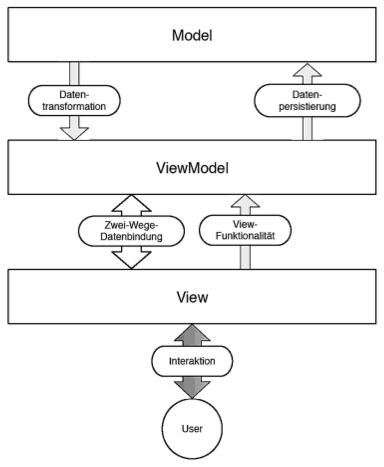
\includegraphics[width=8cm]{kapitel7/bilder/1-model-view-viewmodel}
 \caption{Darstellung der Model-View-ViewModel-Architektur von AngularJS}
 \label{fig:ddmvvmavajs}
\end{figure}

Zu den Kern-Konzepten von AngularJS gehören unter anderen das aus Polymer bekannte Two-Way-Data-Binding, die Controller sowie Direktiven. Das Two-Way-Data-Binding erlaubt die Datenbindung in 2 Richtungen, von Model zu View und umgekehrt. Die dabei entstehenden Änderungen am Model werden automatisch im \ac{DOM} abgebildet und Benutzerinteraktionen innerhalb des Views werden automatisch auf das Model angewendet. Dadurch entfällt die manuelle Manipulation des \ac{DOM}s mithilfe von JavaScript bzw. jQuery, da diese von AngularJS intern mittels der jQuery-lite, einer vereinfachten, leichteren Version von jQuery automatisch vollzogen wird. Die Controllers definieren die Daten und die Logik (ViewModel), die für einen bestimmten View benötigt werden. Sie halten hierfür einen Scope, in dem die Variablen und Funktionen definiert werden, auf die aus dem View heraus zugegriffen werden können soll. Soll mit Hilfe von AngularJS \ac{HTML} um eigene Elemente oder Attribute erweitert werden, so werden hierfür die Direktiven eingesetzt, welche die dafür notwendige Logik kapseln.


\subsection{Vergleich der Intentionen hinter Polymer und AngularJS}\label{vergleich-der-intentionen-hinter-polymer-und-angularjs}

Die Web Components sind eine Sammlung an sich noch in Entwicklung befindenden Technologien und APIs um eigene \ac{HTML}-Elemente zu definieren. Polymer ist eine Library um dies zu vereinfachen und erweitern. Mit Hilfe von Polyfills und zusätzlichen Features kann es \ac{HTML}-Elemente erstellen und sie auch auf Browsern zum Einsatz bringen, welche die nötigen Standards noch nicht unterstützen. AngularJS hingegen stellt APIs auf Framework-Ebene bereit wie Services, Routing oder auch Serverkommunikation. Die Polymer-Library bildet diese Funktionalitäten hingegen nicht ab. Stattdessen muss hierfür auf die mit Polymer entwickelten Iron Elements des Elemente Katalogs zurückgegriffen werden, da diese solche Funktionalitäten bieten. Es kümmert sich mehr darum, das Entwickeln solcher umfangreichen, mächtigen und wiederverwendbarer Komponenten zu ermöglichen. Mit diesen Komponenten wiederum können komplexe Applikationen realisiert werden, wie sie mit AngularJS umgesetzt werden können. Polymer muss daher als eine Library angesehen werden, wobei AngularJS ein komplettes Framework ist. Die durch Polymer erweiterten Web Components entsprechen vielmehr den Direktiven von Angular. Polymer ist also als ein Subset des AngularJS Funktionsumfangs, welcher für das Entwickeln von komplexen Applikationen entworfen ist, anzusehen.


\subsection{Vergleich der Technischen Features}\label{vergleich-der-technische-features}

Dennoch gibt es Features, die sowohl Polymer als auch AngularJS mitbringen. Hierzu zählt das Two-Way-Data-Binding mit einer sehr ähnlichen Syntax sowie die deklarativen Templates zum Definieren von Komponenten-internen Markups. Jedoch überwiegen die Unterschiede beider Funktionsumfänge.

AngularJS ist ein Framework zum Erstellen von \ac{SPA}s und stellt hierfür eine Reihe an Funktionalitäten bereit. Polymer hingegen bietet keine internen Mechanismen für das Strukturieren einer Applikation bereit, stattdessen können die hierfür mit Polymer entwickelten Komponenten eingesetzt werden. Eine mit Polymer realisierte Applikation ist dadurch deklarativ geschachtelt und hierarchisch aufgebaut, was durch das Mediator-Pattern erzwungen wird (siehe Abschnitt 5.1). AngularJS hingegen erfordert keine hierarchische Struktur, da es unter dem Framework nicht nur ein Typ von Komponenten gibt. Dies spiegelt sich auch in dessen Aufbau wieder, da die Definition von Elementen mit AngularJS imperativ in JavaScript erfolgt. Da Definition von Komponenten mit Polymer deklarativ orientiert ist, können diese auch einfacher mit anderen Komponenten, welche nicht mit Polymer erstellt werden, interagieren, da sie normales \ac{DOM} sind. AngularJS hingegen ist nur schwer mit anderen \ac{SPA}-Frameworks zu kombinieren. Des weiteren nutzt Polymer das Shadow \ac{DOM}, bzw. das Shady \ac{DOM}, um Stylesheets und JavaScripte in den Komponenten zu kapseln. In AngularJS wird hierauf verzichtet, da es nur die Daten in dem Scope kapselt. Auch ist das Deployment einer AngularJS-Direktiven einiges umständlicher als mit Polymer, da externe Templates immer relativ zum Projekt oder Domain-Root adressiert werden müssen. Hierzu ist ein zusätzlicher Build-Schritt nötig, der das Template in den Template-Cache schreibt, oder es in die Direktive serialisiert. Zuletzt ist die Browserunterstützung unter AngularJS deutlich breiter - beispielsweise wird der Internet Explorer in Version 8 unterstützt - wodurch es auch bei mehr Projekten in der Produktion eingesetzt werden kann.
